Das vorliegende Kapitel wurde gemeinschaftlich mit drei weiteren Diplomandinnen des BACOSA-Projektes verfasst.  

\subsection{Hiddenseer Boddengewässer (Antje Kerkow, Caroline Lindner)}

\begin{table}[htb]
\caption{Eckdaten für die Standorte entlang des Salzgradienten}
\begin{tabular}{lllrl}
\toprule
 Location				& Date		& Mean Depth	& PSU 			& Salinity Range   \\
 						& 			& ( +M /-M )	& 				& (Venice System 1959)\\
\midrule
Geltinger Bucht 		& June 25	& 1,09 / 0,55	& 9,67 - 10,15 	& $ \alpha $ -mesohaline\\ 
Orther Bucht			& June 26 	& 0,66 / -		& 10,34 - 11,49 & $ \alpha $ -mesohaline\\
Salzhaff 				& June 18 	& 0,86/ 0,30	& 7,80 - 8,30  	& $ \alpha $ -mesohaline\\
\midrule
Vitter Bodden			& July 03 	& 0,83/ 0,62	& 8,02 - 8,28  	& $ \beta $ -mesohaline\\
Griebener Bucht			& July 05 	& 0,87/ 0,65	& 8,11 - 8,86	& $ \beta $ -mesohaline\\
\midrule
Spandowerhagener Wiek 	& July 02 	& 0,84/ -		& 2,70 - 2,76  	& $ \alpha $ -oligohaline\\
\bottomrule
\end{tabular}
\label{Salztabelle}
\end{table}

Die Insel Hiddensee liegt langgestreckt mit einer Nord-Süd-Ausdehnung von 16,6 Kilometern und einer West-Ost-Ausdehnung von maximal 2 Kilometern nordöstlich der Halbinsel Fischland-Darß-Zingst und westlich der Insel Rügen. Auf ihrer Westseite ist sie von der offenen Ostsee, genauer betrachtet von ihrer großräumlichen Einheit Arkonasee, umgeben.

Die Arkonasee hat einen Salzgehalt von 7-9 PSU im Oberflächenbereich und 13 bis 21 PSU am Grund \citep{iow_2014} und wird durch die Darßer Schwelle, einer Erhebung zwischen dem Darß und dem dänischen Gedser, von der westlich angrenzenden Beltsee getrennt \citep{biele_1997}. Die Darßer Schwelle bildet aufgrund einer sprunghaften Änderung des Salzgehaltes eine natürliche ökologische Ausbreitungsgrenze für zahlreiche Organismen \citep{biele_1997}.

Auf der Ostseite Hiddensees befinden sich mit einer Fläche von \unit{170}{\kilo\metre\squared} die flachen westrügenschen Boddengewässer, die Gegenstand dieser Studie waren. Zu ihnen gehören der Vitter Bodden nördlich der Fährinsel mit der angrenzenden Griebener Bucht und der Schaproder Bodden, der sich von der Fährinsel bis zum Gellen, der Südspitze Hiddensees, erstreckt.

Der Einstrom in die Hiddenseer Boddengewässer erfolgt, je nach Windbedingungen, aus unterschiedlichen Richtungen. Im Norden bringt der Rassower Strom Wasser aus dem Libben, dem tiefen Einnschnitt zwischen der Rügener Halbinsel Bug und dem Nordende Hiddensees. An der Südspitze Hiddensees strömt Wasser aus der offenen Ostsee über den Gellenstrom ein, der Barther Strom hingegen bringt durch Zuflüsse stark ausgesüßtes Wasser aus der sonst abgeschlossenen Darß-Zingster-Boddenkette. Ein größerer Zustrom von salzhaltigem Wasser erfolgt bei Einstrombedingungen aus dem Greifswalder Bodden über den Strelasund \citep{leps_1933}.

\cite{hartnack_1926} fand bei 1000 Beobachtungen heraus, dass in der Region insgesamt Winde aus westlicher Richtung dominieren und einen Anteil von \unit{45}{\%} an allen örtlichen Stürmen haben. Dabei kann stark salziges Tiefenwasser aus der Arkonasee über den \unit{4-5}{\metre} tiefen Gellenstrom hereingedrückt werden \citep{leps_1933}. Desweiteren kommen \unit{18}{\%} der Stürme aus Nordwest und \unit{17}{\%} aus Südwest. In der sturmärmsten Jahreszeit, dem Frühling, gewinnen jedoch auch Nord- und Nord-Ost- Stürme an Bedeutung \citep{hartnack_1926}.

Neben den Zugängen zur Ostsee stehen die Hiddenseer Bodden mit der Nordrügenschen Boddenkette in Verbindung, die keinen weiteren Zustrom als über den Vitter Bodden und den Rassower Strom erfährt und die eine geringe Süßwasserzufuhr von 41 Millionen m$^3$ pro Jahr über den Karower Mühlenbach erhält.



\subsubsection{Vitter Bodden (Bozena Nawka, verändert)}


Der Vitter Bodden erstreckt sich zwischen 54\textdegree\ 32\textquotesingle\ 40\dq\ N und 54\textdegree\ 35\textquotesingle\ 51\dq\ N und zwischen 13\textdegree\ 6\textquotesingle\ 29\dq\ E und 13\textdegree\ 9\textquotesingle\ 37\dq\ E \citep{nathansen_2014}. Die \unit{12,4}{\kilo\metre\squared} große Wasserfläche mit einer mittleren Tiefe von \unit{1,4}{\metre} \citep{correns_1976} und einer maximalen Tiefe von \unit{6}{\metre} \citep{biele_1997} liegt im Nationalpark Vorpommersche Boddenlandschaft.

Der Vitter Bodden wird vom nördlichen Teil der Insel Hiddensee mit dem Dornbusch, einem am Ende des Weichselglazials entstandenen Stauchmoränen-Lobus, und von den holozänen Ablagerungen des Alten und Neuen Bessins eingerahmt \citep{katzung_2004}.
Im Süden ist er durch die Fährinsel-Schwelle, ein nur durch die Fahrrinne vertieftes Flachwassergebiet über Geschiebemergel, vom Schaproder Bodden abgegrenzt \citep{mobus_2001}. Im Bereich der Fährinsel hebt sich der Geschiebemergel bis etwa \unit{1}{\metre} unter Flur, während er sich westlich der Fährinsel und im mit holozänen Ablagerungen aus Mudden und Sanden gefüllten Becken des Vitter Boddens auf mehr als \unit{20}{\metre} absenkt \citep{mobus_2001}.

Nach \cite{bachor_2005} beträgt der mittlere Salzgehalt des Vitter Boddens 8,8 PSU und liegt nach dem Venedig-System im $\beta$ -mesohalinen Bereich \citep{gosselck_2011}, was durch eigene Messungen von 8,02 - 8,28 PSU (August und September 2013) bestätigt werden konnte. 

\begin{figure}[htb]
\centering
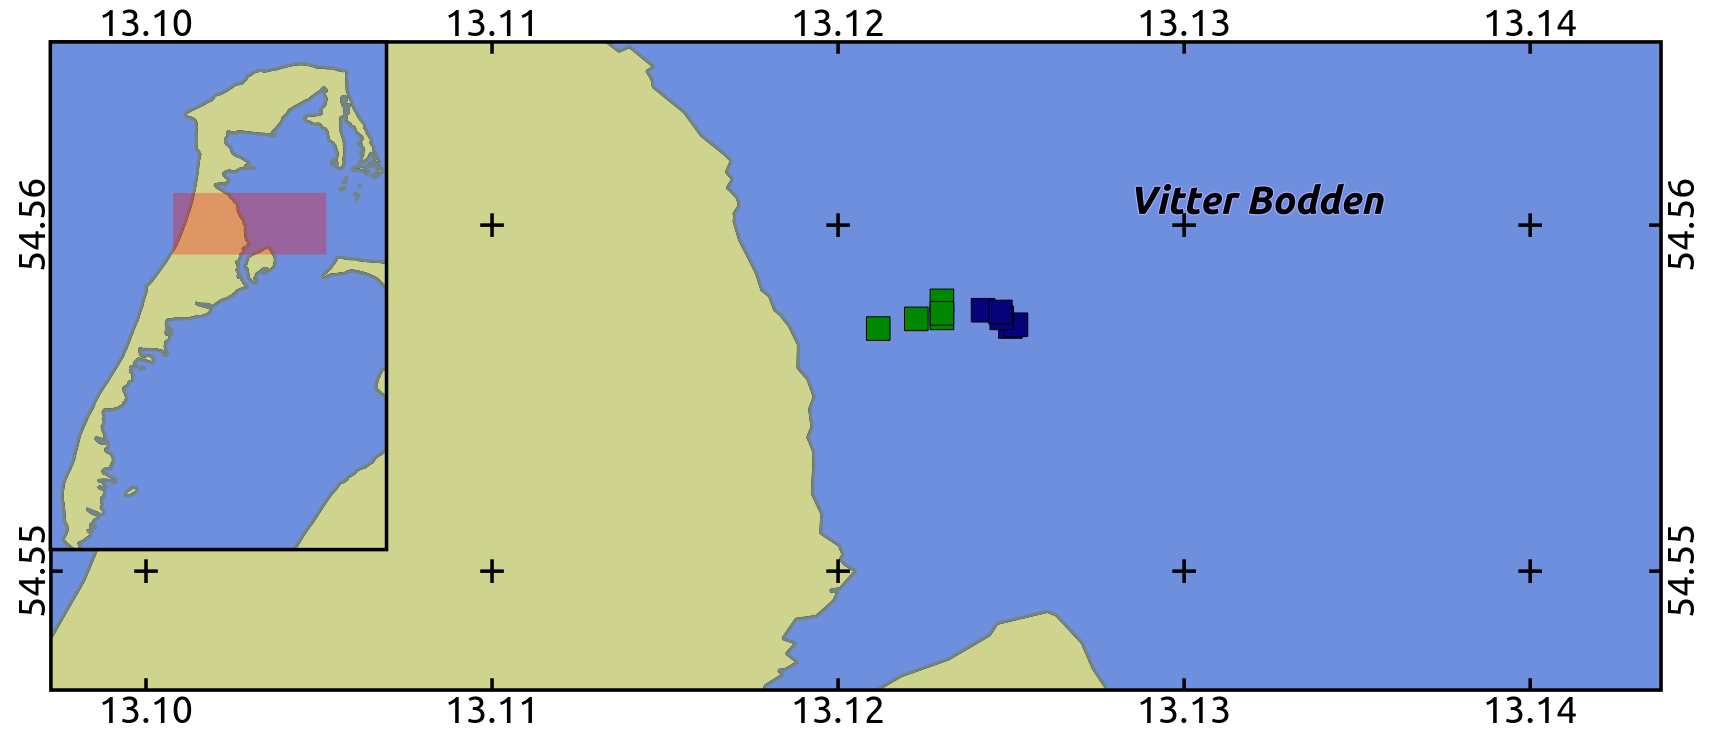
\includegraphics[width=1\textwidth]{images/Vitte.png}
\caption[Probenahmepunkte Vitte]{Probenahmepunkte Vitte; Markierungen: grün = dichte Vegetation, blau = spärliche Vegetation; Maßstab: 1:160.000}
\label{Vitte}
\end{figure}


Die Probennahmestandorte lagen im Flachwasserbereich südlich des Vitter Hafens und nördlich der Fährinsel. Hier ist das Befahren mit motorbetriebenen Wasserfahrzeugen laut Nationalparkverordnung verboten \citep{landesamt_fur_forsten_2002}.

Der makrophytendominierte Standort mit einer mittleren Wassertiefe von \unit{0,83}{\metre} zeigt eine dichte Bedeckung der lose auf dem Boden aufliegenden Braunalge F. vesiculosus f. filiformis. Darin zahreich eingestreut sind winterannuelle Myriophylliden und Parvopotamiden. Der Makrophytenarme Standort hingegen ist auf einer kleinen Sandbank mit einer mittleren Wassertiefe von \unit{0,62}{\metre} gelegen. Hier wachsen vereinzelt Parvopotamiden und die erst später im Jahr aus den Oosporen auskeimenden Chariden. 


\subsubsection{Griebener Bucht (Milena Kafka, verändert)}

Die Griebener Bucht ist Teil des Vitter Boddens und liegt im Nordosten der Insel Hiddensee. Sie ist nur im Süden zum Vitter Bodden hin geöffnet, ansonsten umschlossen von Land. Im Westen liegt der Ort Grieben und im Osten die Bessinsche Schaar \citep{mobus_2000}. Durch die vorwiegenden Westwinde wird  Geschiebemergel aus dem Pleistozän vom Nordufer der Insel abradiert und der enthaltene Sand in südöstliche Richtung durch Hakenbildungen (Alt- und Neu-Bessin) abgelagert \citep{naumann_2012}.

Der Alt-Bessin begann vor 300 bis 500 Jahren zu wachsen, während sich der vorgelagerte Neu-Bessin erst seit etwa 100 Jahren bildet und jährlich \unit{30 bis 60}{\metre} wächst \citep{karge_2007}. Nach \cite{mobus_2000} würden der Bug und der Altbessin zusammenwachsen, wenn für die Schiffahrt zwischen Hiddensee und Rügen die Libben-Fährrinne nicht ausgebaggert werden würde.

Die Griebener Bucht ist im Mittel etwa \unit{1}{\metre} tief \citep{flugge_2004, hendreschke_2009} und als Schutzgebietszone I des Nationalparks ausgewiesen, die das Befahren mit Wasserfahrzeugen, Angeln und Baden untersagt. Ihre Salinität beträgt 8,11 – 8,66 PSU (eigene Messungen von Juli bis September) und gehört nach \cite{gosselck_2011} ebenso wie der Vitter Bodden zur $\beta$ – mesohalinen Zone.

\begin{figure}[htb]
\centering
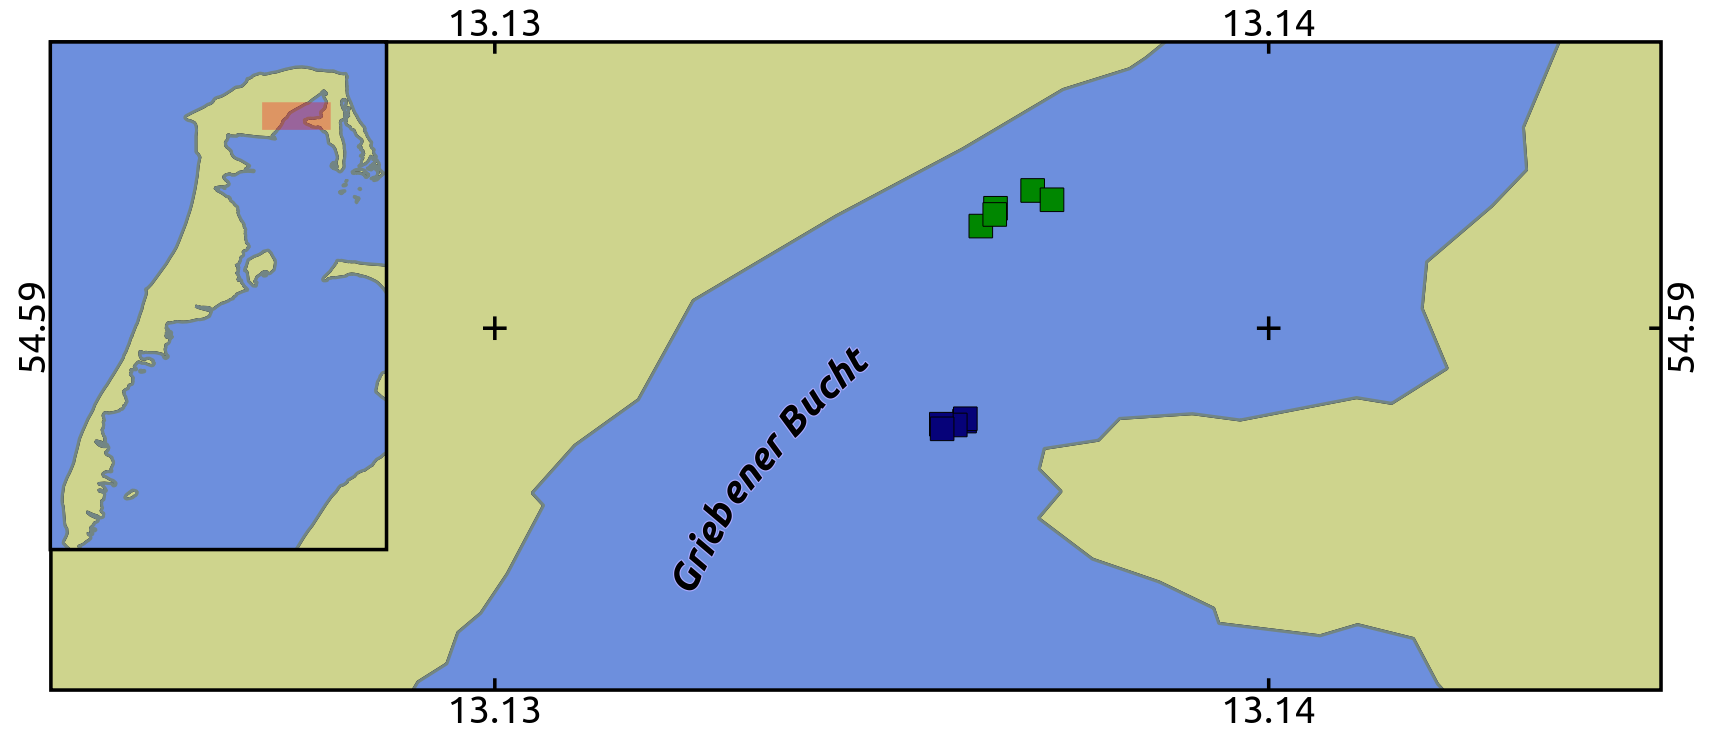
\includegraphics[width=1\textwidth]{images/Grieben.png}
\caption[Probenahmepunkte Griebener Bucht]{Probenahmepunkte Griebener Bucht bei Hiddensee; Markierungen: grün = dichte Vegetation, blau = spärliche Vegetation; Maßstab: 1:6700}
\label{Grieben}
\end{figure}


Der makrophytendominierte Standort für die Probenahmen befand sich \unit{80}{\metre} vom Ufer entfernt am Nordende des Ortes Grieben und die mittlere Wassertiefe dort beträgt \unit{0,87}{\metre}. Hier zeigt sich ein Mosaik aus Parvopotamiden, insbesondere mit \textit{Ruppia cirrhosa} als rasenhaft bestandsbildende Art, aus Chacareen und \textit{Fucus vesiculosus f. balticus}. Der makrophytenarme Standort befand sich mit einer mittleren Tiefe von \unit{0,65}{\metre} \unit{300}{\metre} südöstlich nahe der Ausbuchtung des Alten Bessins. Hier fanden sich vereinzelt Characeen, Parvopotamiden und lose Bällchen des baltischen Blasentangs.



\subsection{Weitere Buchten und Bodden entlang des Salzgradienten}


Es wurden in zwei Bundesländern insgesamt fünf Standorte von West nach Ost ausgewählt: die Geltinger Bucht in der Flensburger Förde, die Orther Bucht südlich der Insel Fehmarn, das Salzhaff in der Wismarer Bucht, der Vitter Bodden bei Hiddensee und die Spandowerhagener Wiek bei Usedom.


\begin{figure}[htb]
\centering
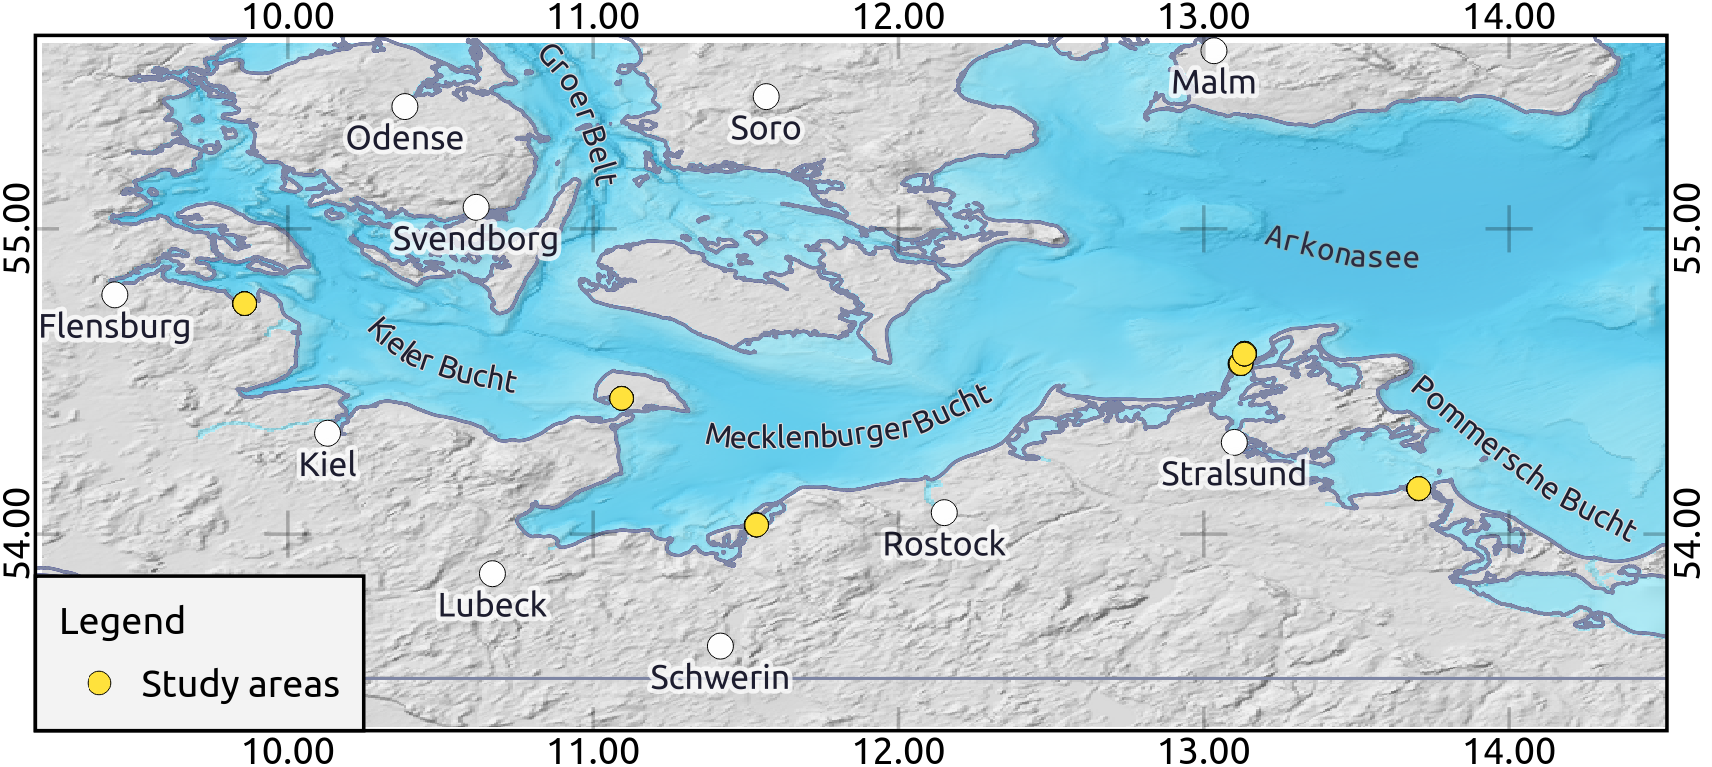
\includegraphics[width=1\textwidth]{images/Uebersicht.png}
\caption[Übersichtskarte der Probenahmestandorte entlang des Salzgradienten]{Probenahmestandorte entlang des Salzgradienten, von links nach rechts: Geltinger Bucht, Orther Bucht, Salzhaff, Hiddensee (Vitter Bodden und Griebener Bucht), Spandowerhagener Wiek; Maßstab: 1:1700000}
\label{Uebersicht}
\end{figure}




\subsubsection{Geltinger Bucht (Antje Kerkow)}


\begin{figure}[htb]
\centering
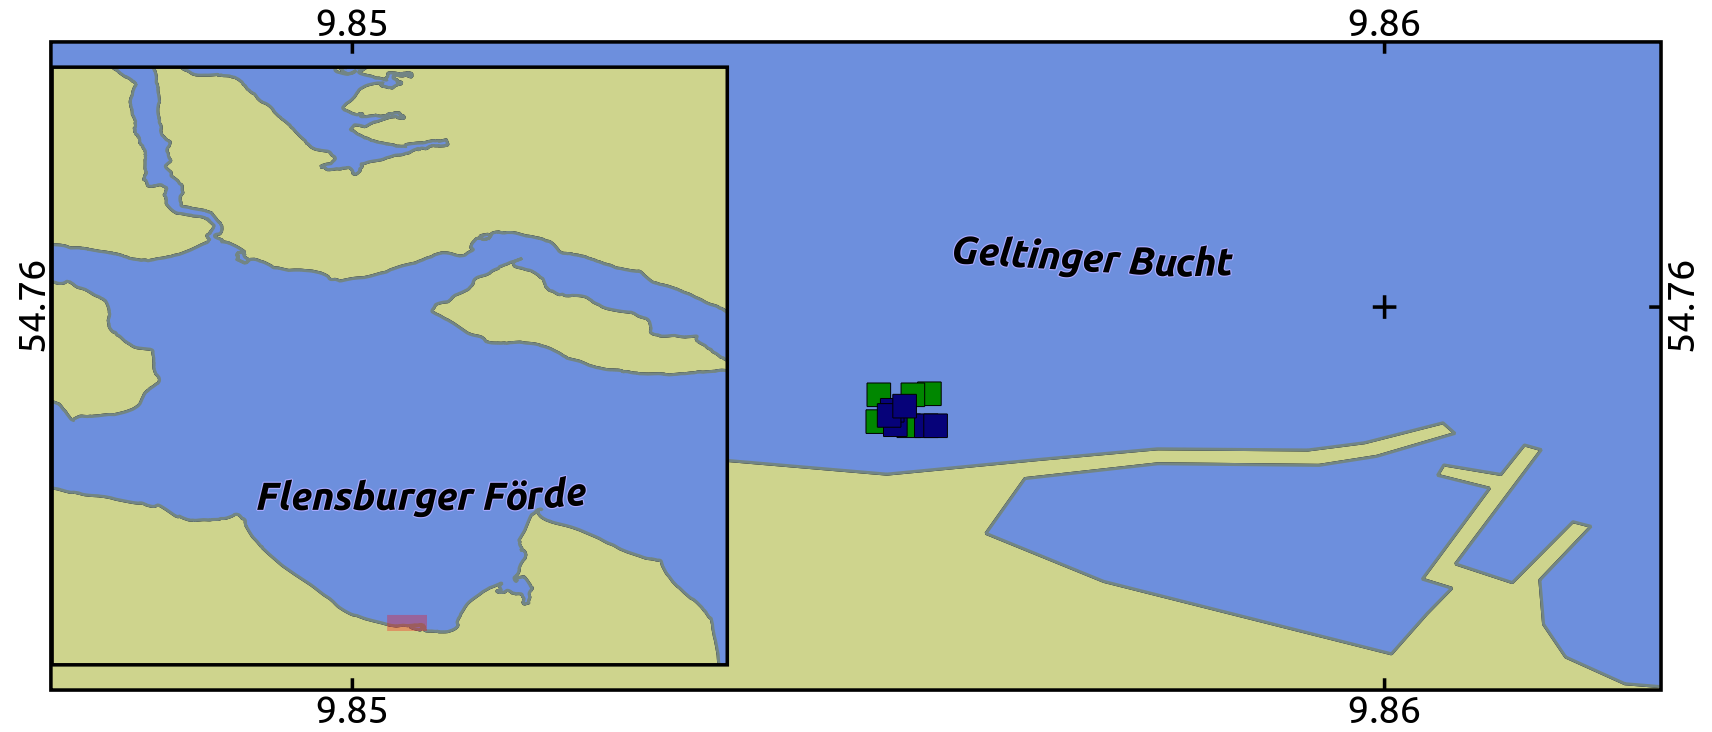
\includegraphics[width=1\textwidth]{images/GB.png}
\caption[Probenahmepunkte Geltinger Bucht]{Probenahmepunkte Geltinger Bucht; Markierungen: grün = dichte Vegetation, blau = spärliche Vegetation; Maßstab: 1:5000}
\label{GB}
\end{figure}


Die Geltinger Bucht ist ein südlicher Ausläufer der Flensburger Außenförde mit einer West-Ost-Ausdehnung von \unit{7,3}{\kilo\metre} und einer Nord-Süd-Ausdehnung von \unit{5}{\kilo\metre}. In ihrem Außenbereich ist sie \unit{20}{\metre} tief \citep{nikulina_2009}, jedoch verfügt sie auch über Steinriffe und ausgedehnte Flachwasserzonen mit Seegrasbeständen   \citep{landesbetrieb_fur_kustenschutz_nationalpark_und_meeresschutz_schleswig-holstein_2013}.

Die Bucht entstand durch den Rückzug des Gletschereises der Weichseleiszeit. Durch Randmöranen entstanden Höhenzüge, die die Bucht in NNW und SSE-Richtung keilförmig einschlossen. Das Grundmoränenbecken dazwischen wurde während des Meeresspiegelanstieges der Litorinatransgression mit Wasser gefüllt \citep{reisch_1997}.

Der Salzgehalt der Geltinger Bucht wird beeinträchtigt durch Stürme, die salziges Ostseewasser über die Holnisschwelle drücken und damit das Tiefenwasser erneuern \citep{nikulina_2009}. Der Süßwassereinstrom  in die Flensburger Förde ist mit \unit{\430}{\kilo\cubic\metre}/Jahr \citep{lanu_2001} dagegen gering.
Das Wasser im tiefen Zentral- und Außenbereich der Bucht ist saisonal geschichtet und wird als meso-polyhalin eingestuft \citep{reimers_2005}. \cite{kandler_1963,exon_1972} und \cite{bluhm_1990} maßen Salzgehaltswerte zwischen 20 und 26 PSU für das Wasser am Grund und 15 bis 20 PSU für das Oberflächenwasser. Die küstennahen Bereiche hingegen werden als mesohalines äußeres Küstengewässer eingestuft. Zum Zeitpunkt der eigenen Untersuchung betrug der Salzgehalt dort zwischen 9,8 und 10,1 PSU.

Der Vegetationsbewuchs der Bucht ist geprägt durch ein dichtes Vorkommen der Arten Fucus vesiculosus und \textit{Ruppia cirrhosa} . Zwischen 1900 und 1950 wurde ebenfalls das Vorkommen von \textit{Chara aspera}, \textit{Chara baltica}, \textit{Lamprothamium papulosum}, \textit{Zannichellia palustris}, \textit{Chorda filum und Fucus serratus} dokumentiert \citep{mertens_2007}.


\subsubsection{Orther Bucht (Antje Kerkow)}

\begin{figure}[htb]
\centering
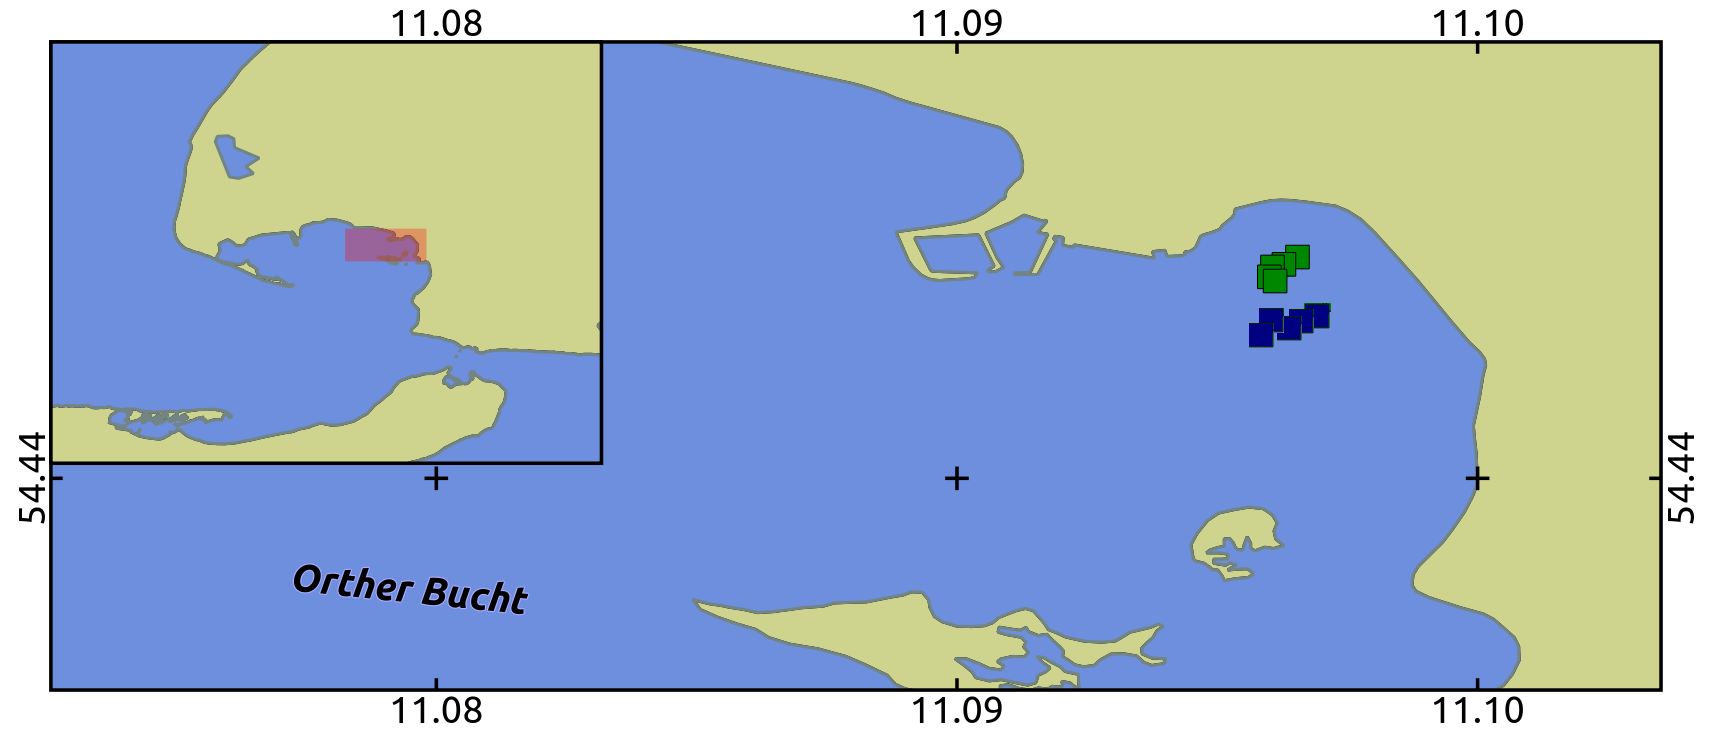
\includegraphics[width=1\textwidth]{images/OB.png}
\caption[Probenahmepunkte Orther Bucht]{Probenahmepunkte Orther Bucht; Markierungen: grün = dichte Vegetation, blau = spärliche Vegetation; Maßstab: 1:10000}
\label{OB}
\end{figure}



Die Orther Bucht liegt mit einer maximalen Tiefe von \unit{4,1}{\metre} \citep{seekarte_fehmarn_sund_kartograph_unbekannt_1902} an der Südwest- Seite der Insel Fehmarn. Die Landschaft in dieser Region ist ein Jungmoränengebiet des Schleswig-Holsteinischen Hügellandes, das von der Weichseleiszeit geformt wurde. Die Bucht misst \unit{4,8}{\kilo\metre} in ihrer West-Ost- und \unit{2,8}{\kilo\metre} in ihrer Nord-Süd-Ausdehnung und wird halb umschlossen von der Nehrungshalbinsel Krummersteert. Diese entstand durch die Abtragung von Sand und Geschiebemergel an der Nordwest-Seite der Insel, wo durch die kräftige Brandung das Material gelockert und mit der Strömung in südliche Richtung abtranspoertiert wird \citep{eschwe_2005}.

Die Orther Bucht wird eingestuft als mesohalines inneres Küstengewässer \citep{reimers_2005} und zeigte zum Zeitpunkt der Untersuchung einen Salzgehalt zwischen 11,0 und 11,5 PSU auf.
Die Vegetation ist sehr artenreich, so bilden wurzelnde Arten, insbesondere Characeen, dichte Bestände bis \unit{1}{\metre} Wassertiefe, während in \unit{2 bis 3}{\metre} Tiefe Zostera marina die bestandsbildende Art ist. In einer umfangreichen Vegetationskartierung 2004 wurden folgende Arten gefunden: \textit{Tolypellia nidifica}, \textit{Chara aspera}, \textit{Chara baltica}, \textit{Chara canescens}, \textit{Lamprothamnium papulosum}, \textit{Ruppia maritima}, \textit{Zostera marina},\textit{ Zannichellia palustris}, \textit{Potamogeton pectinatus}, \textit{Chorda filum} und \textit{Fucus vesiculosus}. Zudem wurden 1951 auch die Arten \textit{Ruppia cirrhosa} und \textit{Fucus serratus} vorgefunden \citep{mertens_2007}.



\subsubsection{Salzhaff (Caroline Lindner, verändert)}

Das Salzhaff liegt im Nordwesten des Bundeslandes Mecklenburg-Vorpommern im Bereich der Koordinaten 54\textdegree\ 2\textquotesingle\ 22\dq\ N bis 54\textdegree\ 5\textquotesingle\ 37\dq\ N und 11\textdegree\ 31\textquotesingle\ 26\dq\ E bis 11\textdegree\ 37\textquotesingle\ 1\dq\ E \citep{nathansen_2014}, nordöstlich der Stadt Wismar und per Luftlinie etwa \unit{35}{\kilo\metre} von Rostock entfernt. Es bildet den Nordostteil der Wismar-Bucht, die zur Mecklenburger Bucht gehört und ist Teil der großräumigen Einheit Beltsee \cite{biele_1997}.

Das Salzhaff wird im Nordwesten durch die Halbinsel Wustrow und die Insel Kieler Ort und im Südwesten durch die Halbinsel Boiensdorfer Werder von der Wismarer Bucht getrennt. Im Süden des Salzhaffs liegt das mecklenburgische Festland.

Die \unit{1,5}{\kilo\metre} breite und \unit{4}{\metre} tiefe Kielung zwischen Kieler Ort und Boiensdorfer Werder verbindet das Salzhaff mit der Wismarer Bucht. Seit 1987 gibt es an der schmalsten Stelle des Kieler Ortes infolge eines sturmbedingten Durchbruchs, der den Haken Kieler Ort von Wustrow trennte, eine zweite Verbindung zur Wismar-Bucht \citep{kohn_1991}.

Das Salzhaff nimmt eine Fläche von \unit{20 bis 22}{\kilo\metre\squared} ein und hat von Südwest nach Nordost eine Länge von \unit{12}{\kilo\metre}. Der vorspringende Tessmannsdorfer Haken teilt das Salzhaff in eine äußere Bucht im Südwesten mit einer Tiefe von bis zu \unit{5}{\metre} und in eine innere Bucht im Nordosten, die eine Tiefe von bis zu \unit{3}{\metre} erreicht \citep{weber_1997}. Die tiefste Verbindung der beiden Buchten bildet der Ellbogen, eine Rinne von etwa \unit{30}{\metre} Breite und \unit{2}{\metre} Tiefe \citep{kohn_1991}.
Die mittlere Tiefe des Salzhaffs liegt bei \unit{2,3}{\metre}. Die maximale Tiefe beträgt \unit{10}{\metre} und befindet sich nordöstlich des Boiensdorfer Werders \citep{kohn_1991}.
Der einzige Süßwasserzufluss ist der Hellbach, der in die innere Bucht mündet, jedoch zu keiner nennenswerten Verringerung des Salzgehaltes führt \citep{weber_1997}. 

Die Mecklenburger Bucht und das Salzhaff unterliegen Salzgehaltsschwankungen, da sie über den Fehmarn Belt mit dem Kattegat und Skagerrak verbunden sind. Daher kamen, wie im Jahr 1994, schon Schwankungen von 8 bis 18 PSU vor. In der Regel liegt der Salzgehalt jedoch über 10 PSU \citep{weber_1997}. Im Juni 2013 konnte dies mit eigenen Messungen von 10,7 PSU im äußeren Salzhaff nachwiesen werden. Das Salzhaff liegt demnach im $ \alpha$ -mesohalinen Bereich \citep{gosselck_2011}. 




\begin{figure}[htb]
\centering
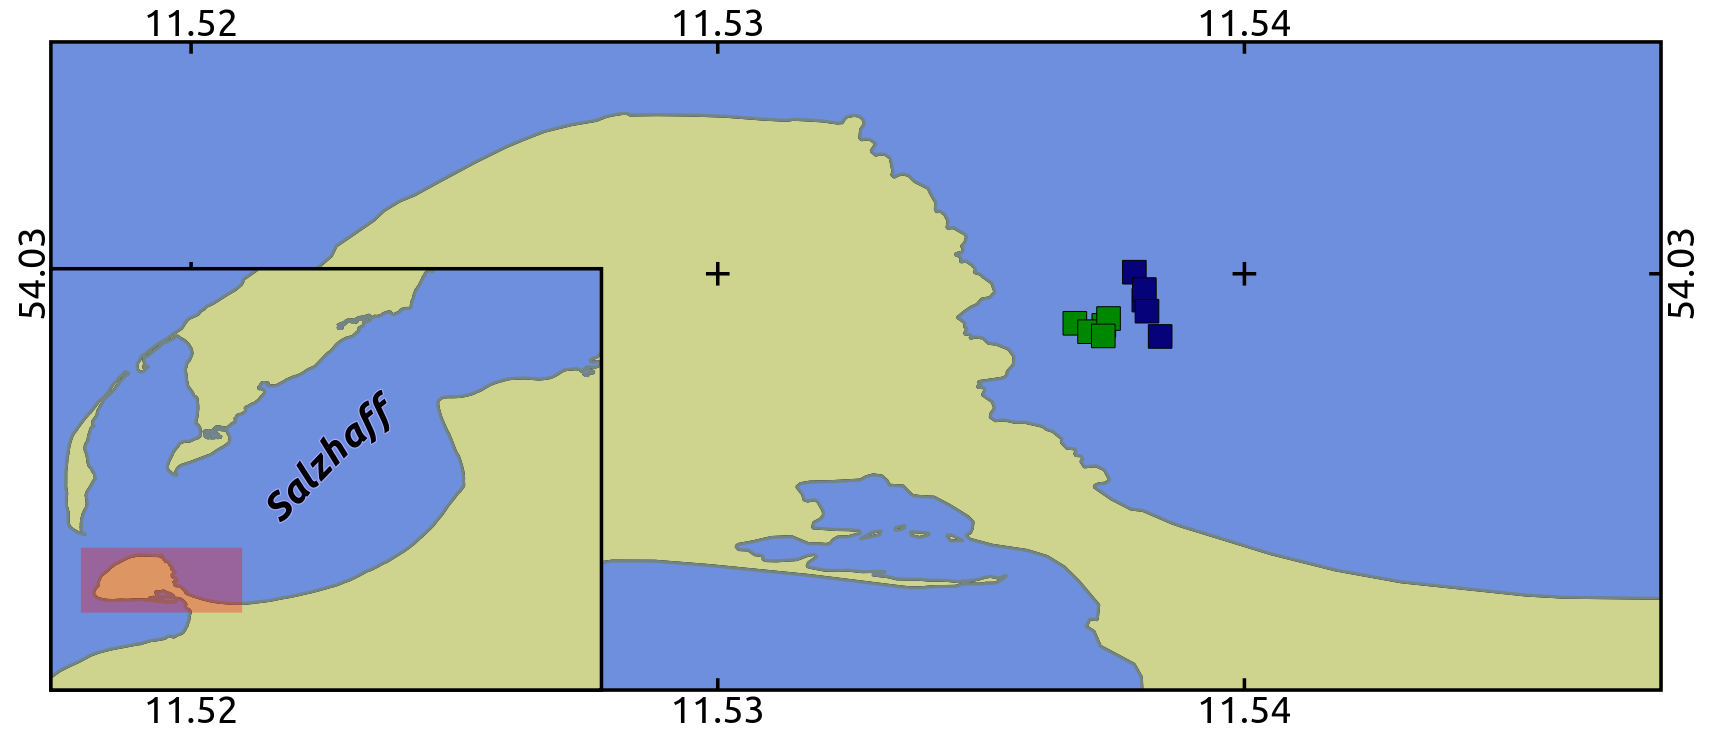
\includegraphics[width=1\textwidth]{images/SH.png}
\caption[Probenahmepunkte Salzhaff]{Probenahmepunkte Salzhaff; Markierungen: grün = dichte Vegetation, blau = spärliche Vegetation; Maßstab: 1:10000}
\label{SH}
\end{figure}



\subsubsection{Spandowerhagener Wiek (Caroline Lindner, verändert)}

Die Spandowerhagener Wiek liegt im Nordwesten der Insel Usedom im Bundesland Mecklenburg-Vorpommern, etwa \unit{22}{\kilo\metre} (Luftlinie) von der Stadt Greifswald entfernt, zwischen den Koordinaten 54\textdegree\ 8\textquotesingle\ 58\dq\ N bis 54\textdegree\ 9\textquotesingle\ 40\dq\ N und 13\textdegree\ 41\textquotesingle\ 55\dq\ E bis 13\textdegree\ 45\textquotesingle\ 6\dq\ E \citep{nathansen_2014}. 
Es handelt sich um eine Bucht, die die Mündung des nördlichen Peenestroms mit dem Greifswalder Bodden verbindet. Sie wird im Osten von der Insel Usedom und im Westen vom vorpommerschen Festland sowie der Insel Struck begrenzt. 

Die Wiek gehört zum Naturschutzgebiet „Peenemünder Haken, Struck und Ruden“ \citep{niedermeyer_2011}.
Das Becken ist flach und wird sowohl von der ausgesüßten Zufuhr der Peene als auch von salzhaltigem Wasser des Greifswalder Boddens gespeist. Es nimmt eine Fläche von \unit{5,4}{\kilo\metre\squared} ein \citep{niedermeyer_2011} und erreicht von Nordwest nach Südost eine maximale Länge von \unit{4}{\kilo\metre}.

Der Greifswalder Bodden ist mit seinen durchschnittlich \unit{5,8}{\metre} etwas tiefer als die flache Spandowerhagener Wiek \citep{meyer_1998}, deren Tiefe bei Struck \unit{2,2}{\metre} beträgt \citep{bartels_1998} und gegenüber im Süden der Wiek bei Freest eine mittlere Tiefe von \unit{1,2}{\metre} aufweist (Buckmann et al 1998). Der Flachwasserbereich ist durch die Fahrrinne der Peene und der etwa \unit{4}{\metre} tiefen Rinne zum Kühlwasserkanal des ehemaligen Kernkraftwerks Nord durchzogen \citep{gosselck_2007}.

Je nach Wasserstand kommt es im Bereich der Peenemündung und des Peenestroms zu salzhaltigem Einstrom aus dem Greifswalder Bodden oder zum Ausstrom von Wasser geringer Salinität aus der Peene \citep{buckmann_1998}. Dadurch kann der Salzgehalt im nördlichen Peenestrom und damit in der Spandowerhagener Wiek zwischen 1 und 8,5 PSU erheblich schwanken \citep{meyer_1998}.

Im Bereich der Spandowerhagener Wiek bei dem Ort Freest wurde eine sprunghafte Abnahme des Salzgehaltes von etwa 6 bis 9 PSU im Greifswalder Bodden auf 3 PSU im Mündungsgebiet festgestellt \citep{gunther_1998}. Untersuchungen im Rahmen des BACOSA-Projektes im Juli 2013 am Westufer nahe Spandowerhagen ergaben einen Salzgehalt von 2,7 PSU. Damit liegt die Spandowerhagener Wiek im $\alpha$ - oligohalinen Bereich.



\begin{figure}[htb]
\centering
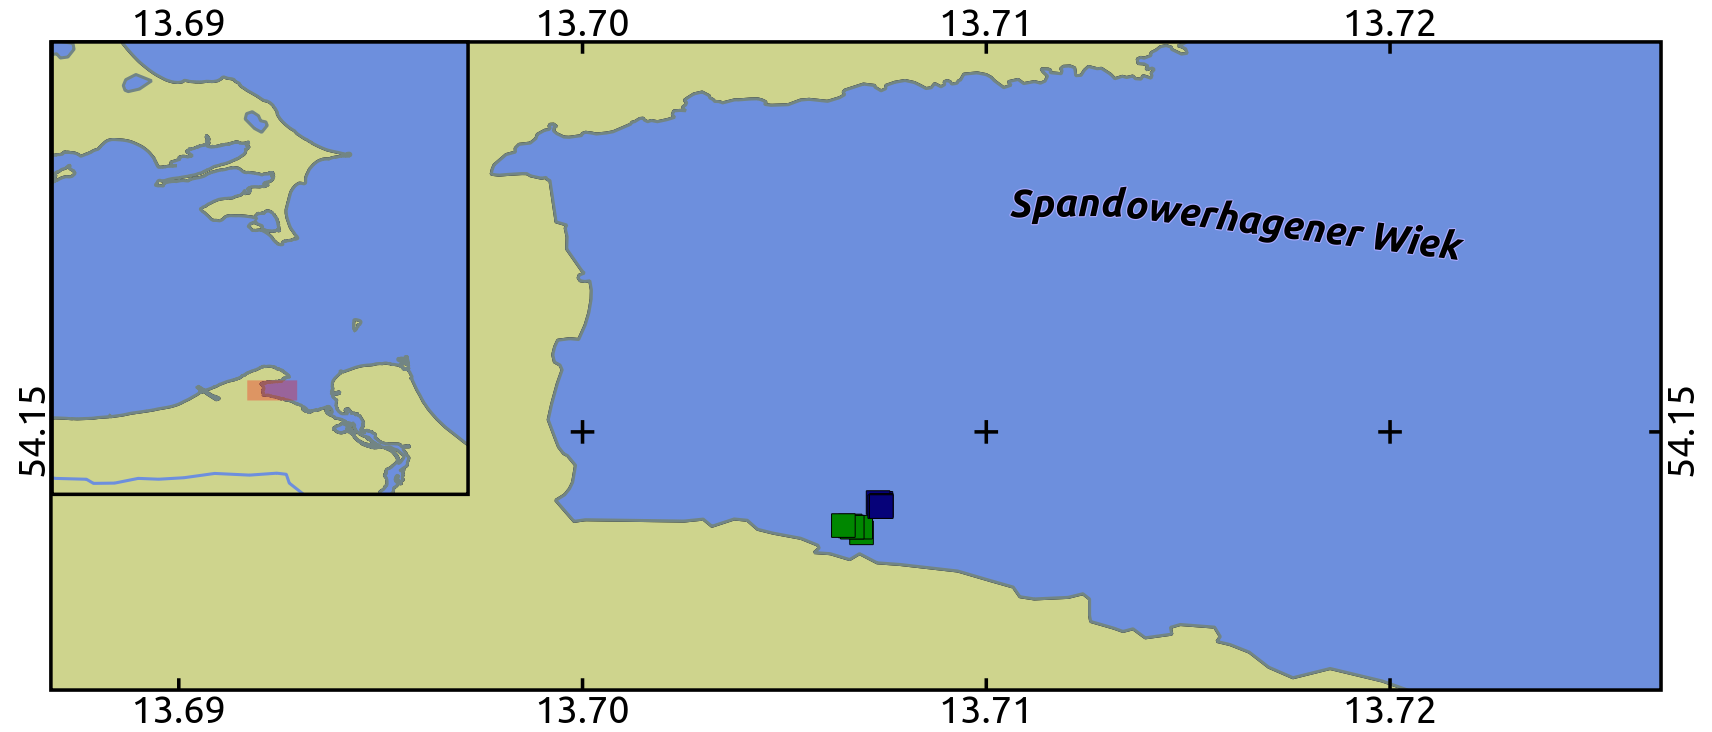
\includegraphics[width=1\textwidth]{images/SW.png}
\caption[Probenahmepunkte Spandowerhagener Wiek]{Probenahmepunkte Spandowerhagener Wiek; Markierungen: grün = dichte Vegetation, größere vegetationsfreie Flächen sind nicht vorhanden; Maßstab: 1:13000}
\label{SW}
\end{figure}



